%!TEX root = ../marisa-thesis.tex
\chapter{Application: Chemical Combinatorics}
Combinatorics can be used to explore different areas of study.  The chemical bonds represented by Lewis Structures can be evaluated for the total number of closed walks.  Moreover, the closed walks may present a pattern that can be utlizied for the different molecular structures which may create a pattern.  This pattern may be used to find a general equation to find the total number of closed walks, which can be applied to all the hydrocarbons being tested. %\ce{CH4}

\section{Methane}
%\chemfig{C(-[:0]H)(-[:90]H)(-[:180]H)(-[:270]H)}
\begin{figure}[h]
         \centering
         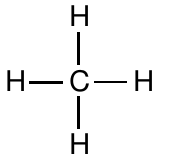
\includegraphics[width = 2.0in]{23.png}
         \caption{\small{The molecular structure of methane.}}
 \end{figure}

  Methane is a molecule that is part of the alkane group.  The representation of the molecular structure is presented in Figure 4.1.  
   \par This can be viewed as a graph to count the total number of walks throughout the structure.
  %\item
  \\
  \\Therefore, the graph contains 4 edges and 5 vertices represented by bonds (for edges) and the elemental symbol (for vertices.)
  \\We can represent the structure as a mathematical graph we recognize.
 \begin{figure}[h]
     \centering
     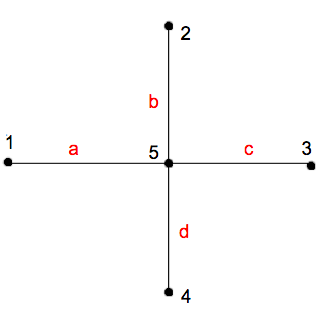
\includegraphics[width=0.30\textwidth]{hydrocarbon1.png}
     \caption{\small{The graphical representation of the methane molecular structure.}}
 \end{figure}
 \\
 \\Figure 4.2 illustrates the edges annoted as letters and the vertices annotated with numbers. To find the total number of walks, the adjacency matrix must be calculated and its determinant found.
\\\\The adjacecy matrix shows how many walks from one vertex to another vertex has.  Here the adjacency matrix is showing the total number of walks with length 1.\\
We can explore the number of walks throughout the molecule. From $v_5$ we notice that it has the most access over the other vertices. It can use all of the edges that are part of the molecule.  The outlying vertices cannot reach each other without taking the edge to the center vertex first.  Noticing this, we can make propositions about it. 
\begin{proposition}
    Total number of closed walks of length 3 does not exist on the methane graph.
\end{proposition}
\begin{proof}
    We are given the methane graph and wish to prove that a closed walk of length 3 does not exist.  We will do this via contradiction and assume that the closed walk of length 3 does exist.  \par \textbf{Case 1: Outlying vertex} Assuming the closed walk of length 3 exists, then I can take any vertex and have it make that closed walk.  Let us take vertex ${v_n}$.  We leave ${v_n}$ via edge ${e_i}$.  Thus, one walk is used.  Due to the structure of the graph, we have four options to choose from to take another edge.  We choose ${e_j}$.  ${e_j}$ leaves us at another vertex, ${v_m}$.  We only have one more walk left.  Because of the graphs structure we must take the same edge, ${e_j}$ to return to the center vertex.  We have used our three walks and have not returned to our beginning vertex, ${v_n}$.  Thus, we have reached our contradiction. \par \textbf{Case 2: Center vertex} Asssume we start with the center vertex, ${v_p}$. ${v_p}$ has four edges to choose from.  ${v_p}$ commits to an edge.  Since there are no cycles within the graph, the walk must return to ${v_p}$.  Thus, there are two walks already used and we already returned to our beginning vertex.  Therefore, we have reached a contradiction. \\
\end{proof}
The proof is characteristic of all vertices within the graph.  We also know from the earlier chapters that there cannot be an odd total number of closed walks. This proposition furthers this claim. 
\\ In addition, we know that there are connections between the center and the rest of the vertices.  Thus, we can propose the impact of the center vertex, as follows:

\begin{proposition}
    The total number of closed walks of length 4 from the outlying vertices will be equal to the number of closed walks of length 2 from the center vertex.
\end{proposition}
\begin{proof}
    We are given the methane graph and we wish to prove the total number of closed walks of length 4 is equal to the total number of closed walks of length 2.  There are a total number of 4 closed walks for the length of 2.  \par \textbf{Case 1: Outlying vertex} Since, the first and last spot are already taken because we have to take the same edge back as we started with.  Thus, there are only two more spots left.  Those steps are controlled by the center vertex. Once a step is commited to, the same step must be taken back.  Thus, the inner walks of length 4 are the closed walks of length 2 from the center vertex. 
\end{proof}
\begin{theorem}
    The hydrocarbons will not contain odd number of closed walks.
\end{theorem}
\begin{proof}
    Referring back to chapter 2 proposition 2.1.1
\end{proof}
\begin{lemma}
    The hydrocarbons will only contain even number of closed walks that will be controlled by the center vertices. 
\end{lemma}
Let us explore our propositions. The total number of closed walks for even length can be found using the equation as a foundation. 
\begin{equation}
    W_{G}^1(2m)= W_G^5(2m-2)
\end{equation}
Equation 4.1 demonstrates the total even closed walks from vertex 1. We can add these total even closed walks for every vertex to find the total number of even closed walks.
\begin{align*}
    W_{G}^i(2m) = W_{G}^1(2m) + W_{G}^2(2m)+... W_{G}^5(2m)
    W_{G}^i(2m) = 2^{2m+1}
\end{align*}
Therefore, we can create an equation that establishes an overall definition for total even closed walks within a methane molecule.

\begin{equation}
    W_{G}^i(2m) = 2^{2m+1}
\end{equation}
Equation 4.2 can possibly used later to reveal a pattern within ethane - $C_2H_6$.

\section{Ethane}
There are three other hydrocarbons that can be explored for closed number of walks.  Analyzing each may yield a pattern that facilitates the prediction of how a molecular structure forms, and how the structure looks. \\
    \par

    \begin{figure}
        \begin{center}
    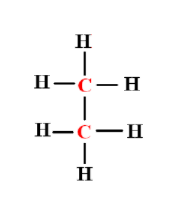
\includegraphics[width=0.30\textwidth]{ethane.png}
    \end{center}
    \caption{\small{The molecular structure of the ethane.}}
    \end{figure}
This structure contains the same symmetry as methane, but with an added "methane" shape, that allows the same conditions to apply. 
\\
\par
There are two cases that can be examined for the ethane molecule
\begin{enumerate}
    \item Staying inside the structure formally known as methane -- which we already have the formula for. 
    \item The closed walks must include new edges represented by the labelling (\textbf{\textcolor{red}{a, b, d}}) that are from the "methane" part of the molecule with a walk that begins at the "ethane" part of the molecule.
\end{enumerate}
     We can create a graphical illustration, like the methane graph made previously, to help follow the walks we wish to count from particular vertices using particular edges that are labeled.  For simplicity, we will continue to add to the graph of the methane molecule, therefore having the same labelled edges and vertices to help seek out patterns from one part of the hydrocarbon to the other.

-- add picture here -- 

When including new edges and the original case of remaining inside the ``methane'' shape, the equation below arises:

\begin{equation}
    W^C_{G_{1,4}} = (W^l_{G_{1,4}}(4)-1) \times 6 +W^C_{G_{1,4}}(6)+W^l_{G_{1,4}}(6)
\end{equation}

\section{Propane}
We are going to explore propane to determine if there are any patterns that are similar to the previous 2 hydrocarbons.\\

\par To continue our search further we want to find patterns from the methane and ethane molecules that are present in the propane molecule. First, we have two cases, which are:
\begin{enumerate}
    \item The center vertex
    \item The outlying vertices (which are the same due to symmetry therefore we can use one to represent all)\\
\end{enumerate}
\begin{figure}
        \begin{center}
    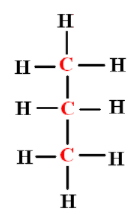
\includegraphics[width=0.30\textwidth]{propane3.png}
    \end{center}
    \caption{\small{The molecular structure of the propane.}}
    \end{figure}
Let us examine. We already know due to our earlier proposition that there will not be any total number of odd closed walks within the molecule. Thus, we will examine the total number of even closed walks.

\par Analyzing a walk of length 2 we will discover that the pattern is the same as all of the other hydrocarbons thus far. We only have one edge that can move away from the beginning vertex and the same edge to return to it. Therefore, we can move on to determine any patterns in a closed walk of length 4.
\par Looking at a closed walk of length 4 starting at vertex 1, we can see that we begin with only one option to move away from $v_1$ to get to $v_4$.  Moreover, $v_4$ has 3 options to be chosen from. After the choice is made, there is only one choice that can be made to get back to $v_4$ and leave that particular vertex, and only one more walk left to return back to $v_1$. We can discern that the final 2 walks within the length 4 walk is actually a walk of length 2. We can generalize this discovery, but to be sure, we can confirm this pattern with one more even closed walk. Let us look at an even closed walk of length 6.

\par For the condition of a closed walk of length 6, we have two cases.
\begin{enumerate}
    \item Staying within the partial graph that only contains $v_4$ as the center and 4 oulying vertices that are directly connected to it.
    \item Moving to $G_{2,6}$ which is the ethane molecule.
\end{enumerate}

For case 1, we already know that there will only be one option to leave $v_1$ and only option to return to $v_1$.  Therefore, the first and last spots of our walk are already taken.  Thus, we are left with a closed walk of length 4 from vertex 4. This is because $v_1$ -- similar to other outlying vertices-- are connected to $v_4$ and must return back to $v_4$ to ensure the walk will be closed (will return to the beginning vertex.) \\

For case 2, there still contains a closed walk of length 4, with the beginning and ending walks only containing one option. \\
\par Therefore, we can draw a conclusion from these patterns to generalize all hydrocarbon structures.

\begin{proposition}
     Let $i$ be a leaf in $G_{C,H}$ and $a_{i,j}$ $\in$ $E(G_{C,H})$. Then, 
         $W^i_{G_{C,H}}(2m)$ = $W^j_{G_{C,H}}(2m-2)$
 \end{proposition} 
Thus, we can use this equation to represent all outlying vertices for every hydrocarbon, because the shape never changes.  Therefore, the properties of the hydrocarbon never change and the symmetry remains.
 \begin{equation}
     W^i_{G_{C,H}}(2m) = W^j_{G_{C,H}}(2m-2)
 \end{equation}